\section*{سوال ۶}

تفاوت «مدل ایجاد نرم‌افزار» مانند آبشاری یا حلزونی با «متدولوژی ایجاد نرم‌افزار» مانند XP یا RUP در چیست؟

انجمن علمی دانشکده مهندسی کامپیوتر خواستار «مدلی» برای برگزاری رویدادهای دانشجویی است. در طراحی این مدل، باید به ویژگی‌های زیر توجه شود:
\begin{itemize}
	\item حق‌الزحمه‌ای به نیروهای برگزارکننده پرداخت نمی‌شود.
	\item احتمال عدم انجام وظایف توسط برگزارکنندگان به دلیل عدم تعهد رسمی.
	\item دانشجویان وقت محدودی دارند.
	\item موضوعات رویداد حول مباحث رشته‌ی مهندسی کامپیوتر است.
	\item هدف اصلی، یادگیری و سپس لذت بردن از کار تیمی است.
	\item مخاطبین عمدتاً دانشجویان و دانش‌آموزان هستند.
\end{itemize}

\subsection*{موارد مورد توجه در طراحی}
\begin{itemize}
	\item جامعه مخاطبین
	\item ثبت‌نام مخاطبین
	\item جذب داوطلبین برگزاری
	\item انتخاب افراد داوطلب
	\item تخمین هزینه‌ها
	\item حامی مالی
	\item تبلیغات و برندینگ
	\item خط زمانی رویداد
	\item هماهنگی‌های اداری
\end{itemize}

با توجه به مدلی که در قسمت قبل تهیه کرده‌اید، متدولوژی‌ای برای برگزاری یک رویداد خاص طراحی کنید. این متدولوژی باید موقعیت خاصی را در نظر بگیرد و به صورت دقیق به ویژگی‌های آن بپردازد.

\section*{جواب سوال ۶}

تفاوت بین
\textbf{مدل ایجاد نرم‌افزار}
و
\textbf{متدولوژی ایجاد نرم‌افزار}
به نحوه‌ی دستورالعمل‌ها، فرآیندها، تکنیک‌ها و ابزارهایی برمی‌گردد که در هر کدام استفاده می‌شوند. بیایید این دو را با یکدیگر مقایسه کنیم:

\subsection*{مدل ایجاد نرم‌افزار:}

مدل ایجاد نرم‌افزار به الگوهای کلی مراحل و فعالیت‌های لازم برای توسعه نرم‌افزار اشاره دارد. این مدل‌ها معمولاً رویکردی سطح بالا به فرآیند توسعه نرم‌افزار دارند و می‌توانند مفاهیم مختلفی را در بر بگیرند که تیم‌ها باید دنبال کنند.

\begin{itemize}
	\item \textbf{آبشاری \lr{(Waterfall)} :}
یک مدل خطی و ترتیبی است که در آن هر مرحله باید کاملاً تمام شود قبل از اینکه مرحله بعدی شروع شود. مثال: ابتدا تحلیل نیازمندی‌ها، سپس طراحی سیستم، پس از آن پیاده‌سازی، تست و نهایتاً نگهداری.
	\item \textbf{حلزونی \lr{(Spiral)} :}
مدل حلزونی نیز مراحل آبشاری را دنبال می‌کند، اما با یک رویکرد تکراری که اجازه می‌دهد بازگشت به مراحل قبلی برای بهبود و اصلاح وجود داشته باشد. در هر دور، یک نسخه جدید و بهبود یافته از نرم‌افزار ساخته می‌شود.
\end{itemize}

\subsection*{متدولوژی ایجاد نرم‌افزار:}

متدولوژی ایجاد نرم‌افزار نه تنها مراحل کلی فرآیند توسعه را تعریف می‌کند، بلکه تکنیک‌ها، ابزارها، و دستورالعمل‌های دقیقی را برای هر مرحله ارائه می‌دهد. متدولوژی‌ها معمولاً بسیار جامع‌تر هستند و می‌توانند شامل توصیه‌هایی برای برنامه‌ریزی، تخمین زمان، مدیریت پروژه، توسعه و نگهداری باشند.

\begin{itemize}
	\item \textbf{\lr{XP (eXtreme Programming)} :}
یک متدولوژی چابک است که بر توسعه تکراری، برنامه‌ریزی مداوم، و بهبود مستمر تاکید دارد. همچنین، این متدولوژی بر توسعه به شیوه‌ی جفتی، تست محور و داشتن بازخورد مداوم از مشتری تأکید می‌کند.

	\item \textbf{\lr{RUP (Rational Unified Process)} :}
این متدولوژی یک فرآیند تکراری و افزایشی است که به تیم‌ها کمک می‌کند تا معماری نرم‌افزار را به خوبی تعریف کنند و مدیریت ریسک را در فرآیند توسعه ادغام کنند. RUP مجموعه‌ای از بهترین شیوه‌ها را در تمام جنبه‌های توسعه نرم‌افزار معرفی می‌کند.
\end{itemize}

بنابراین با توجه به تعریف‌هایی که داشتیم، تفاوت عمده در این است که مدل‌های توسعه نرم‌افزار بیشتر به الگوی کلی و توالی فعالیت‌ها توجه دارند، در حالی که متدولوژی‌های توسعه نرم‌افزار جزئیات دقیق‌تری از نحوه اجرای هر مرحله و اصول راهنما را ارائه می‌دهند و اغلب شامل راهنمایی‌های عملی‌تر و مشخص‌تر برای تیم‌های توسعه می‌شوند.

\begin{itemize}
	\item \textbf{تمرکز بر فرآیند:} مدل‌های ایجاد نرم‌افزار بیشتر روی فرآیند توسعه متمرکز هستند. آنها مراحل و توالی عمومی فعالیت‌های مورد نیاز برای تولید نرم‌افزار را تعریف می‌کنند.
	\item \textbf{جامعیت پایین‌تر:} مدل‌هایی مانند آبشاری یا حلزونی معمولاً دستورالعمل‌های مشخص و جزئی برای پیاده‌سازی فرآیندها ارائه نمی‌دهند. آن‌ها چارچوب‌های کلی هستند که نحوه به دنبال کردن هر مرحله را به تیم‌های توسعه واگذار می‌کنند.
	\item \textbf{انعطاف‌پذیری کمتر:} مدل‌ها مانند آبشاری سفت و سخت‌تر هستند و تغییرات را در میانه‌ی پروژه به خوبی تحمل نمی‌کنند.
	\item \textbf{پیش‌بینی‌پذیری:} این مدل‌ها به دلیل ترتیب مشخص شده‌شان پیش‌بینی‌پذیری بیشتری در مراحل توسعه فراهم می‌آورند، که می‌تواند برای مدیریت پروژه مفید باشد.
\end{itemize}

\subsection*{بررسی دقیق‌تر متدولوژی‌های ایجاد نرم‌افزار (مانند XP یا RUP ):}

\begin{itemize}
	\item \textbf{تمرکز بر جزئیات:} متدولوژی‌ها جزئیات دقیق‌تری از نحوه اجرای هر مرحله از فرآیند توسعه را فراهم می‌آورند، شامل روش‌ها، ابزارها، و دستورالعمل‌های خاص.
	\item \textbf{جامعیت بالاتر:} متدولوژی‌ها مجموعه‌ای از بهترین شیوه‌ها، قالب‌ها و استانداردهای صنعتی را ادغام می‌کنند که می‌تواند شامل توصیه‌های متعدد برای تمام جنبه‌های توسعه نرم‌افزار باشد.
	\item \textbf{انعطاف‌پذیری بیشتر:} متدولوژی‌ها مانند XP طراحی شده‌اند تا به تیم‌ها اجازه دهند به صورت چابک و با قابلیت پاسخگویی بالا به تغییرات پاسخ دهند.
	\item \textbf{تاکید بر بهبود مداوم:} متدولوژی‌ها اغلب شامل مکانیزم‌هایی برای بازنگری و بهبود مداوم فرآیندها هستند.
\end{itemize}

\subsubsection*{مثال:}

\begin{itemize}
	\item مدل آبشاری به شما می‌گوید که ابتدا نیازمندی‌ها را جمع‌آوری کنید، سپس طراحی کنید، پس از آن کدنویسی، سپس تست و در نهایت به تحویل محصول بپردازید. این یک توالی خطی و غیرقابل بازگشت است.
	\item متدولوژی RUP ، که یک متدولوژی تکراری و تدریجی است، به شما می‌گوید که چگونه باید نیازمندی‌ها را با استفاده از تکنیک‌های خاص جمع‌آوری کنید، چطور باید معماری را مدل‌سازی کنید، چگونه ریسک‌ها را مدیریت کنید و چطور فرآیندهای کدنویسی و تست را به صورت تکراری و با ادغام تغییرات انجام دهید.
\end{itemize}

\subsection*{ارائه‌ی مدل برای برگزاری رویدادهای انجمن علمی}

همان‌طور که می‌دانیم،
\lr{4MAT Learning Model}
مدلی برای طراحی تجربیات یادگیری و تدریس است که توسط دکتر برنیس مک‌کارتی توسعه یافته است. این مدل مبتنی بر این است که یادگیری در چهار فاز اصلی رخ می‌دهد: وابستگی (Why) ، تفکر (What) ، عملی (How) ، و ابداع (If) . با این حال، می‌توانیم از اصول این مدل برای طراحی و پیاده‌سازی مدل برگزاری رویدادهای دانشجویی استفاده کنیم. حالا در این مرحله، ما به تعریف دقیق هر مرحله از مدل خودمون می‌پردازیم و بررسی می‌کنیم که در هر مرحله چه کارهایی باید انجام شود و سپس تسک‌های تعریف شده در هر رویداد انجمن علمی را، اساین می‌کنیم به مراحل با توجه به تعاریفشان.

\subsubsection*{وابستگی (چرا؟ – Why ) :}

\textbf{هدف‌گذاری و انگیزه:}
در این مرحله، لازم است که انگیزه‌های برگزاری رویداد را مشخص کرده و به اعضا و داوطلبان بفهمانیم که چرا مشارکت آن‌ها اهمیت دارد. این کار با ارائه مزایای شرکت در رویدادها، مانند یادگیری و تجربه کار تیمی، انجام می‌شود. به‌خصوص باید در فرم جذب استف‌ها و صحبت‌های دبیر-نایب‌دبیر رویدادها با افراد خارج از رویداد، باید به مزایای شرکت در رویداد اشاره شود و همچنین برگزارکنندگان اصلی رویدادها باید تلاش کنند تا مزایای زیادی ایجاد کنند برای حضور در تیم برگزاری رویداد و تمرکزشان را روی یادگیری مهارت‌های نرم و سخت قرار دهند.

\subsubsection*{تفکر (چه چیزی؟ – What ) :}

\textbf{اطلاعات و داده‌ها:}
ارائه اطلاعات کلیدی در مورد رویداد، موضوعات، مخاطبین هدف، و فرآیند برگزاری به داوطلبان و شرکت‌کنندگان. این شامل توزیع دستورالعمل‌های دقیق، برنامه‌ها و مواد آموزشی است. در واقع، در این مرحله اطلاعات کلی و جزئی مربوط به نحوه‌ی شرکت در رویداد، نحوه‌ی استف شدن در رویداد، جزئیات شیوه‌ی برگزاری رویداد، مکان برگزاری‌ها، اطلاعات مربوط به شبکه‌های اجتماعی و باقی موارد، به اطلاع مخاطبان می‌رسد. این روند از طریق سوشال مدیاهای رویداد و همچنین کلامی می‌تواند شکل بگیرد.

\subsubsection*{عملی (چگونه؟ – How ) :}

\textbf{فرایند برگزاری:}
توسعه یک نقشه عملی برای برگزاری رویداد که شامل جذب داوطلبین، ثبت‌نام، تخمین هزینه‌ها، جذب حامی مالی، تبلیغات و برندینگ، خط زمانی رویداد و هماهنگی‌های اداری می‌شود. در این فاز باید دستورالعمل‌های عملی و واضحی برای هر یک از این بخش‌ها ارائه شود. این بخش خیلی دقیق به روند برگزاری رویداد می‌پردازد و نحوه‌ی برگزاری را مشخص می‌کند. در این‌جاست که دبیر-نایب‌دبیر رویدادها، درباره‌ی موارد مختلف مربوط به رویدادها تصمیم‌گیری می‌کنند و برنامه‌ی شیوه‌ی برگزاری را می‌ریزند. 

\subsubsection*{ابداع (اگر چه چیزی؟ – If ) :}

\textbf{بازخورد و بهبود:}
در این مرحله، فرصتی برای ارزیابی و بازاندیشی فراهم می‌شود. پس از هر رویداد، تیم برگزاری باید دور هم جمع شوند و در مورد آنچه خوب پیش رفت و چه چیزهایی نیاز به بهبود دارند بحث کنند. این مرحله همچنین فرصتی برای بررسی احتمالات جدید و نوآوری‌های احتمالی در رویدادهای آتی است. جلسات بازبینی رویداد در این مرحله برگزار می‌شوند و مستندات در این مرحله به کار می‌آیند. در واقع تیم مستندسازی با هدف این مرحله تشکیل می‌شود در رویدادها.

\begin{figure}[h]
	\centering
	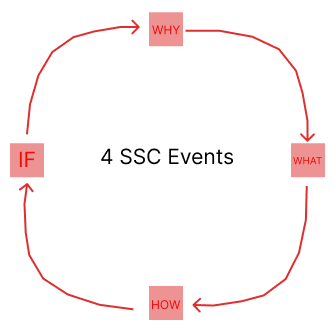
\includegraphics{pic1.png}
	\label{fig:label4}
\end{figure}

در طراحی یک مدل برگزاری رویدادهای انجمن علمی، موارد زیر باید با دقت مورد توجه قرار گیرند تا اطمینان حاصل شود که هر جنبه از رویداد به درستی برنامه‌ریزی و اجرا می‌شود:

\subsubsection*{جامعه مخاطبین}
\begin{itemize}
	\item تعیین جامعه مخاطبین هدف با توجه به موضوع و هدف رویداد.
	\item شناخت دقیق نیازها و علایق مخاطبین برای طراحی محتوای مرتبط و جذاب.
\end{itemize}

\subsubsection*{ثبت‌نام مخاطبین}
\begin{itemize}
	\item ایجاد فرم‌های ثبت‌نام آسان برای استفاده که تمامی اطلاعات لازم را جمع‌آوری کند.
	\item طراحی سیستم ثبت‌نام آنلاین و اتوماسیون برای کاهش اشتباهات و تسهیل پروسه ثبت‌نام.
\end{itemize}

\subsubsection*{جذب داوطلبین برگزاری}
\begin{itemize}
	\item تعیین نقش‌ها و مسئولیت‌های داوطلبین و ایجاد فراخوان عمومی برای جذب داوطلبین.
	\item انتشار فراخوان در شبکه‌های اجتماعی، تابلوهای اعلانات، و دیگر پلتفرم‌ها برای رسیدن به جامعه گسترده‌تری از داوطلبین.
\end{itemize}

\subsubsection*{انتخاب افراد داوطلب}
\begin{itemize}
	\item برگزاری مصاحبه‌های کوتاه و ارزیابی‌های مهارتی برای انتخاب داوطلبین مناسب.
	\item تاکید بر تیم‌سازی و تعامل برای اطمینان از همکاری موثر داوطلبین.
\end{itemize}

\subsubsection*{تخمین هزینه‌ها}
\begin{itemize}
	\item تهیه یک جدول بودجه دقیق که تمام هزینه‌های مورد انتظار را پوشش دهد.
	\item بررسی منابع مالی موجود و تعیین استراتژی برای تامین کسری بودجه احتمالی.
\end{itemize}

\subsubsection*{حامی مالی}
\begin{itemize}
	\item شناسایی و جذب حامیان مالی با ارائه پروپوزال‌های قانع‌کننده و مزایای تبلیغاتی متقابل.
	\item مذاکره با حامیان بالقوه و ایجاد قراردادهای شفاف و متعهدانه.
\end{itemize}

\subsubsection*{تبلیغات و برندینگ}
\begin{itemize}
	\item طراحی یک کمپین تبلیغاتی جامع که شامل رسانه‌های دیجیتال، چاپی و شاید برودکست باشد.
	\item ایجاد یک هویت برند قوی و به یادماندنی برای رویداد که در تمامی مواد تبلیغاتی به کار گرفته شود.
\end{itemize}

\subsubsection*{خط زمانی رویداد}
\begin{itemize}
	\item تدوین یک برنامه زمانی دقیق برای تمام جنبه‌های رویداد، از پیش‌برنامه‌ریزی تا پیگیری پس از برگزاری.
	\item انتخاب تاریخ و زمان مناسب که با رویدادهای دیگر تداخل نداشته باشد و برای اکثر مخاطبین قابل دسترس باشد.
\end{itemize}

\subsubsection*{مکان برگزاری}
\begin{itemize}
	\item انتخاب مکانی مناسب با ظرفیت کافی و امکانات لازم برای اجرای رویداد.
	\item بررسی دسترسی به مکان، امنیت، پارکینگ و سایر عوامل لجستیکی.
\end{itemize}

\subsubsection*{برنامه‌ریزی محتوا}
\begin{itemize}
	\item تعیین اسپیکرها، موضوعات ارائه، کارگاه‌ها، و بحث‌های پنلی.
	\item طراحی برنامه‌ای جذاب و متنوع که مخاطبین را ترغیب به مشارکت فعال کند.
\end{itemize}

\subsubsection*{لوجستیک و تدارکات}
\begin{itemize}
	\item تدارک تجهیزات لازم مانند سیستم‌های صوتی/تصویری، وسایل ارتباطی، و نیازهای پذیرایی.
	\item ایجاد تیم لوجستیکی برای مدیریت و نظارت بر جزئیات در طول رویداد.
\end{itemize}

\subsubsection*{ارزیابی و بازخورد}
\begin{itemize}
	\item طراحی نظرسنجی‌ها و فرم‌های بازخورد برای ارزیابی تجربه شرکت‌کنندگان.
	\item برنامه‌ریزی برای جمع‌آوری و تجزیه و تحلیل داده‌های به دست آمده به منظور بهبود رویدادهای آتی.
\end{itemize}

\subsubsection*{مدیریت بحران}
\begin{itemize}
	\item پیش‌بینی مشکلات احتمالی و تهیه برنامه‌های جایگزین برای حوادث ناگهانی.
	\item تعیین فرایندهای ارتباطی برای مواجهه با شرایط اضطراری. 
\end{itemize}

با دقت به این موارد و انعطاف‌پذیری در برابر تغییرات احتمالی، یک انجمن علمی می‌تواند رویدادهای موفق و ماندگاری را برگزار کند که به ارتقای دانش و همکاری بین اعضا کمک می‌کند.

در بخش‌بندی بالاتر ذکر شده بود که هر کدوم از این موارد در کدوم یک از ۴ بخش مدل قرار می‌گیرند، برای همین در زیر هر کدام، فقط به توضیح روند کلی تعیین شده در مدل برای هر کدام، پرداختیم.

\subsection*{تعریف متدولوژی برگزاری یک رویداد خاص}

\subsubsection*{تعریف موقعیت و ویژگی‌های رویداد}
\begin{itemize}
	\item نوع رویداد: وبینار تخصصی با پنل‌های بحث و کارگاه‌های آموزشی.
	\item هدف رویداد: افزایش آگاهی درباره چالش‌های امنیت سایبری و ارائه راهکارهای نوآورانه.
	\item مخاطبین هدف: متخصصان IT ، دانشجویان حوزه تکنولوژی، شرکت‌های فعال در حوزه امنیت سایبری.
	\item زمان بندی: یک رویداد 3 روزه در ماه دسامبر.
	\item پلتفرم: برگزاری آنلاین از طریق پلتفرمی مانند Zoom یا Webex با قابلیت‌های امنیتی بالا.
\end{itemize}

\subsubsection*{تحلیل نیازمندی‌ها و محدودیت‌های رویداد}
\begin{itemize}
	\item تکنولوژی مورد نیاز: نیاز به سرورهای قوی برای پشتیبانی از وبینار و پخش زنده.
	\item محتوای آموزشی: جذب سخنرانان مطرح، مدرسان مجرب و ارائه‌دهندگان محتوا.
	\item بودجه: تعیین بودجه متناسب با هزینه‌های تکنولوژیک و تبلیغات.
	\item زمانبندی: هماهنگی با تقویم‌های بین‌المللی تا با رویدادهای مشابه تداخل نداشته باشد.
\end{itemize}

\subsubsection*{برنامه‌ریزی جامع برای برگزاری}
\begin{itemize}
\item \textbf{برنامه رویداد} تدوین جدول زمانی دقیق برای سخنرانی‌ها، پنل‌ها و کارگاه‌ها.
\item \textbf{تبلیغات} طراحی کمپین‌های تبلیغاتی موثر در شبکه‌های اجتماعی و انجمن‌های تخصصی.
\item \textbf{حامیان مالی} جذب حامیان مالی با ارائه بسته‌های تبلیغاتی اختصاصی.
\item \textbf{ثبت‌نام} ایجاد سیستم ثبت‌نام آسان و امن برای شرکت‌کنندگان.
\end{itemize}

\subsubsection*{پیاده‌سازی و اجرای رویداد}
\begin{itemize}
	\item فنی: راه‌اندازی و آزمایش زیرساخت‌های فنی قبل از رویداد.
	\item مدیریت داوطلبین: تربیت و هماهنگی تیم پشتیبانی برای راهنمایی و پاسخگویی به شرکت‌کنندگان.
	\item پشتیبانی زنده: تأمین پشتیبانی فنی به صورت لحظه‌ای در طول برگزاری رویداد.
\end{itemize}

\subsubsection*{ارزیابی و بازبینی پس از اتمام رویداد}
\begin{itemize}
	\item نظرسنجی‌ها: اجرای نظرسنجی‌ها فوراً پس از پایان هر بخش و در پایان رویداد.
	\item تحلیل داده‌ها: بررسی داده‌های جمع‌آوری شده برای فهمیدن نقاط قوت و ضعف رویداد.
	\item گزارش‌دهی: تهیه گزارش کامل از رویداد و به اشتراک‌گذاری با سخنرانان و شرکت‌کنندگان.
	\item طرح بهبود: توسعه طرح‌های بهبود برای اجرای موفق‌تر رویدادهای بعدی.
\end{itemize}

\subsubsection*{توسعه محتوا و مواد آموزشی}
\begin{itemize}
	\item \textbf{تهیه محتوا:} همکاری با سخنرانان برای تهیه اسلایدها، ویدئوها و مواد دوره‌های آموزشی.
	\item \textbf{دسترسی به مواد:} فراهم کردن دسترسی به محتوا برای شرکت‌کنندگان قبل و بعد از رویداد.
	\item \textbf{تنوع بخشی:} اطمینان حاصل کردن از تنوع بخشی به مواد آموزشی برای پوشش دادن به انواع یادگیری.
\end{itemize}

\subsubsection*{برقراری ارتباط و شبکه‌سازی}
\begin{itemize}
	\item \textbf{فضاهای تعاملی:} ایجاد فضاهای تعاملی مجازی برای ارتباط بین شرکت‌کنندگان و سخنرانان.
	\item \textbf{فعالیت‌های شبکه‌سازی:} برنامه‌ریزی برای فعالیت‌های شبکه‌سازی مانند جلسات Q\&A و میزگردها.
	\item \textbf{استفاده از رسانه‌ها:} تشویق شرکت‌کنندگان به استفاده از هشتگ‌های رویداد در شبکه‌های اجتماعی.
\end{itemize}

\subsubsection*{مدیریت ریسک و مسائل امنیتی}
\begin{itemize}
	\item \textbf{برنامه‌ریزی برای امنیت:} تضمین امنیت سایبری و حفظ حریم خصوصی در طول برگزاری وبینار.
	\item \textbf{مدیریت ریسک:} شناسایی و ارزیابی ریسک‌های احتمالی و تدوین برنامه‌های مدیریت بحران.
\end{itemize}

\subsubsection*{تبلیغات و ارتقاء رویداد}
\begin{itemize}
	\item \textbf{تبلیغات پیش از رویداد:} اجرای کمپین‌های هدفمند برای جذب حداکثری شرکت‌کنندگان.
	\item \textbf{مشارکت‌های استراتژیک:} همکاری با انجمن‌ها و سازمان‌های مرتبط برای افزایش دید و اعتبار.
	\item \textbf{تبلیغات درون برنامه‌ای:} استفاده از فرصت‌های درون رویداد برای ترویج برنامه‌های آتی.
\end{itemize}

\subsubsection*{پایان‌بخش و تحویل محتوا}
\begin{itemize}
	\item \textbf{ارائه گواهی‌نامه‌ها:} صدور گواهی شرکت برای شرکت‌کنندگان و سخنرانان.
	\item \textbf{بایگانی و دسترسی:} ارائه دسترسی به ضبط جلسات برای بازبینی در آینده.
	\item \textbf{پیگیری پس از رویداد:} ارسال ایمیل‌های تشکر و دعوت برای فیدبک به شرکت‌کنندگان.
\end{itemize}

\subsubsection*{نتیجه‌گیری}
با دنبال کردن این متدولوژی، می‌توان یک رویداد مجازی موفق برگزار کرد که نه تنها در زمان برگزاری، بلکه قبل و بعد از آن نیز تاثیر مثبت و دوامی درازمدت بر جامعه هدف خود داشته باشد.